\section{POSIX IO Overheads}
\label{sec:posix-overheads}

In our examination of the overheads of POSIX IO we benchmark and analyze
CephFS, the file system that uses Ceph's object store (RADOS) to
store its data/metadata and a metadata server cluster to service client requests
more quickly.  During this process we discovered, based on the analysis and
breakdown of costs, that durability and consistency have high overhead but we
urge the reader to keep in mind that this file system is an implementation of
one set of design decisions and our goal here is to highlight the effect that
those decisions have on performance.  At the end of each subsection we compare
the approach to ``decoupled namespaces", the technique in related work that
detaches subtrees from the global namespace to relax consistency/durability
guarantees. 

%The RPCs are also serialized because the
%metadata server is single threaded; although na\"{\i}ve, this design is common
%because of the complexity of multi-threaded metadata
%servers~\cite{konstantinos:pdsw2014-lustre-metadata}.  

\subsection{Durability}
\label{sec:durability}

\begin{figure*}[t]
  \centering
  \begin{subfigure}[b]{.32\linewidth}
      \centering
      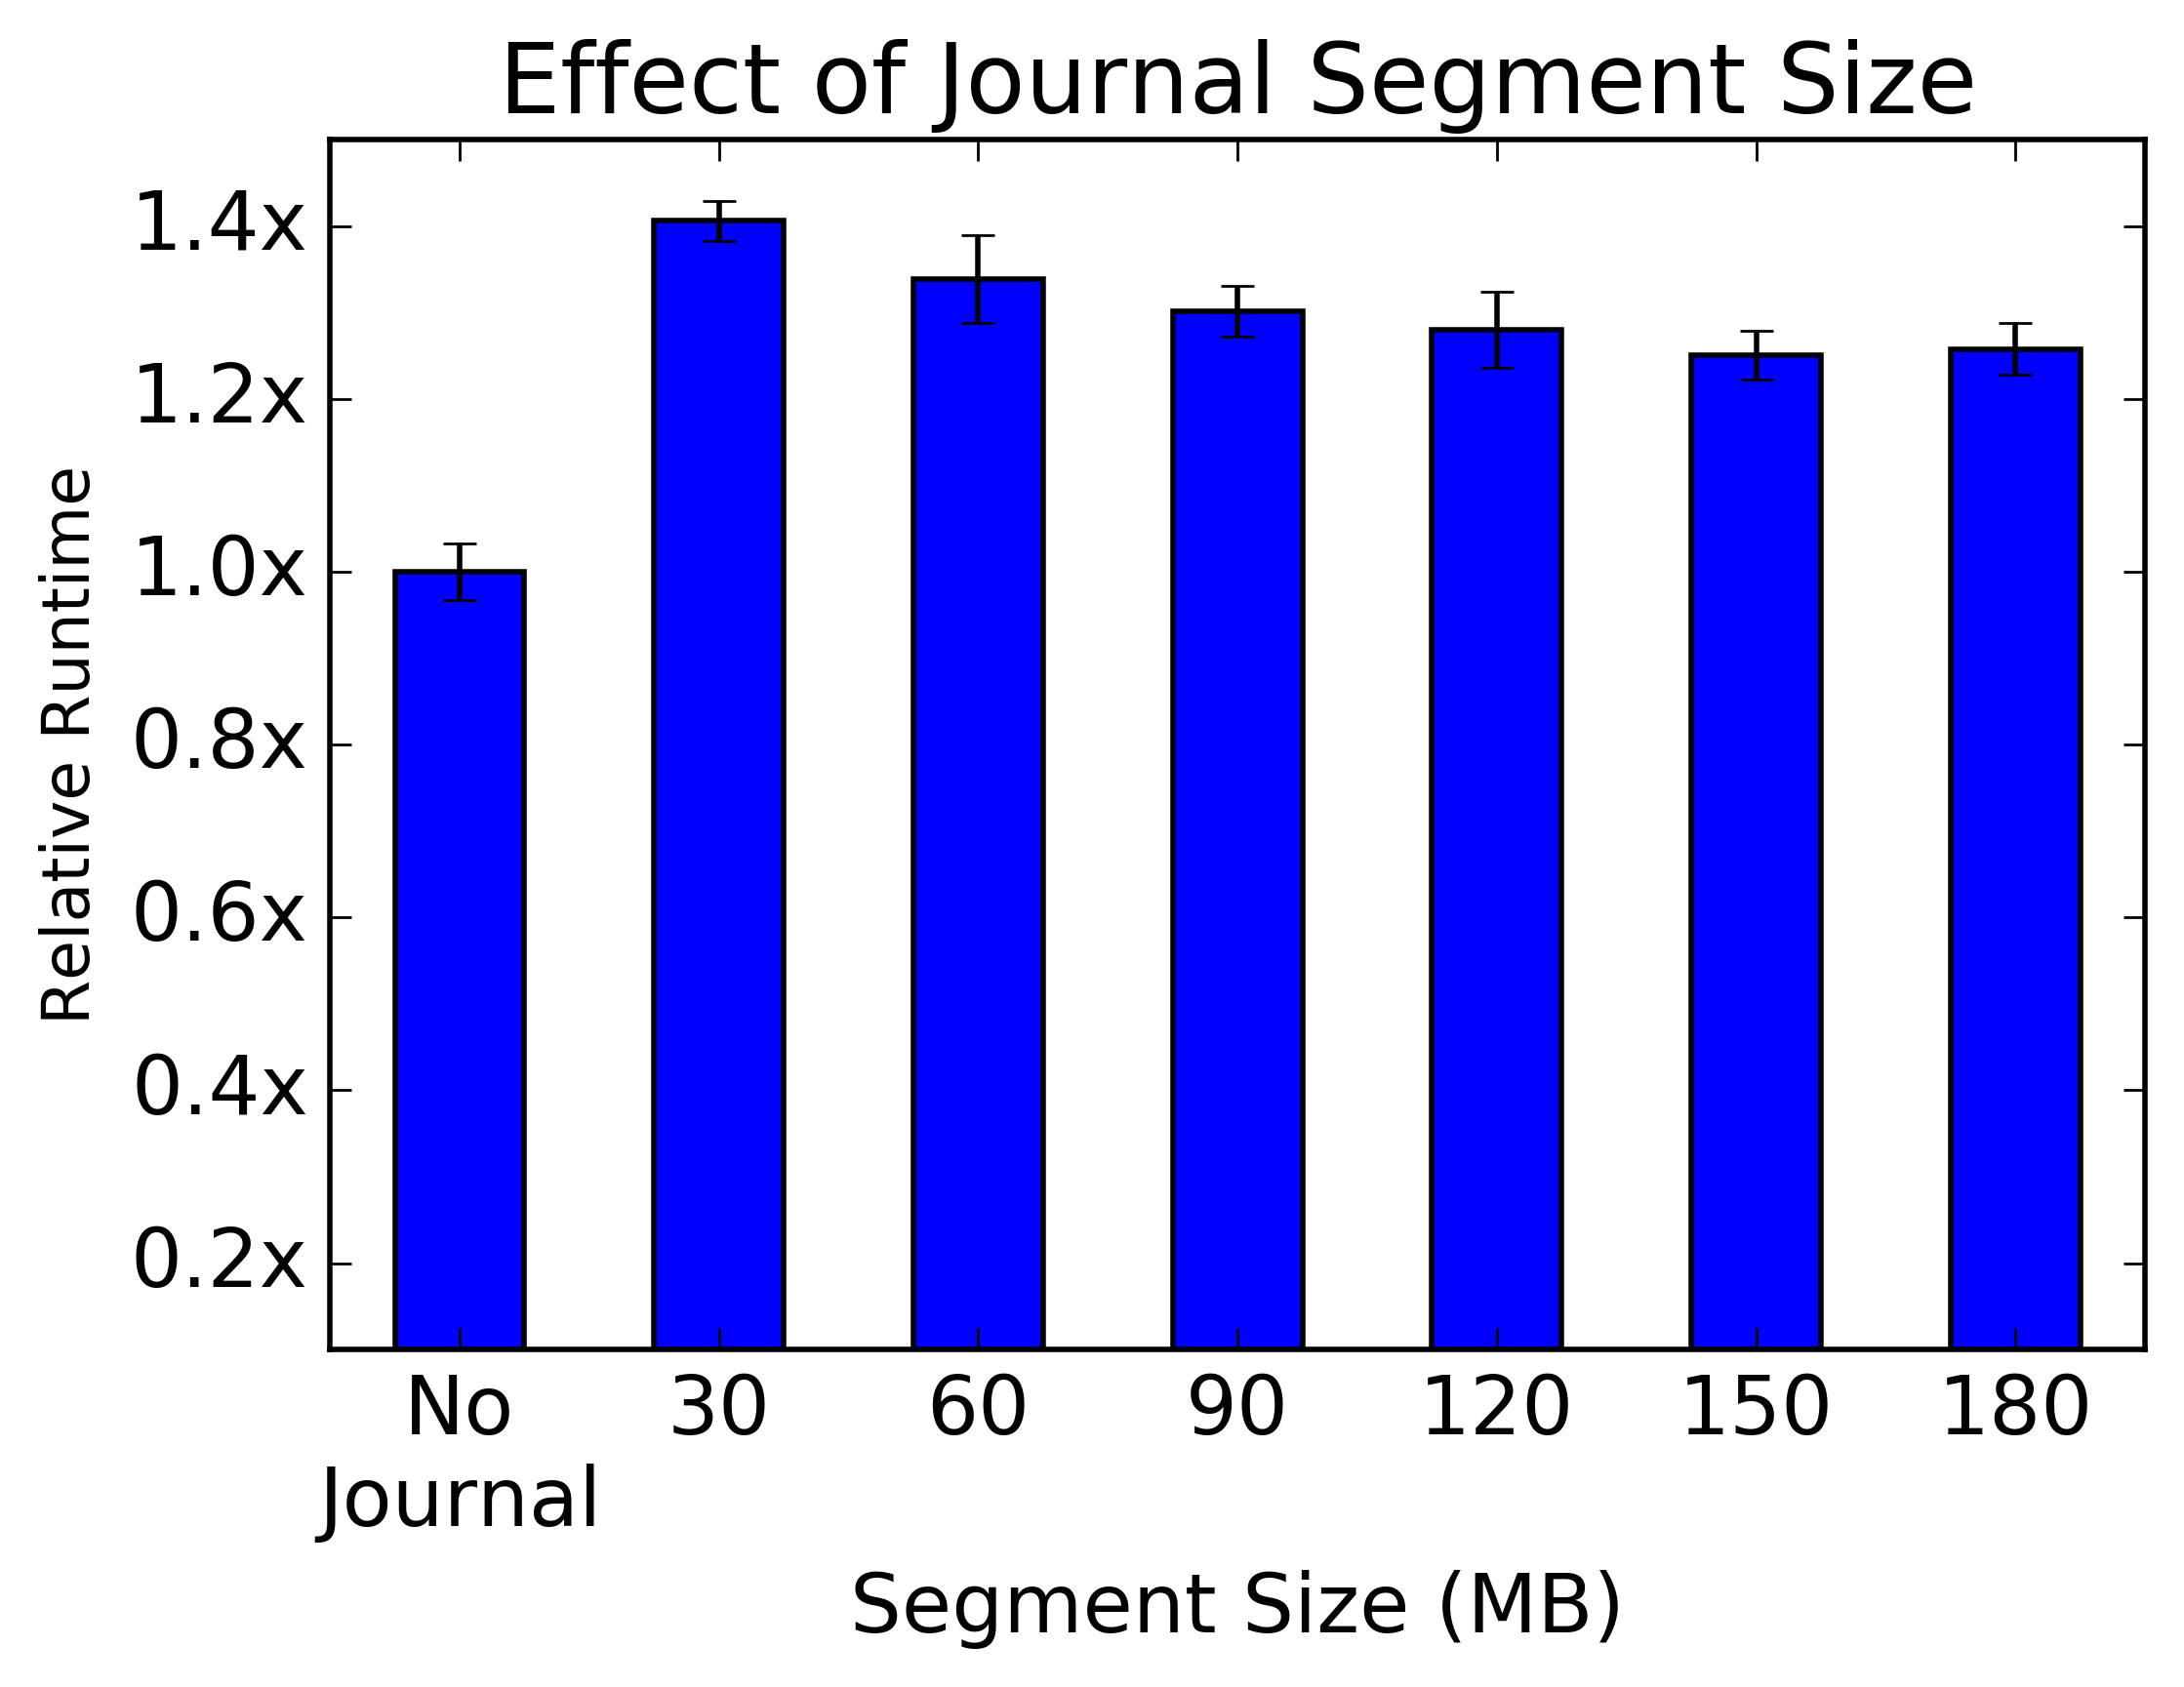
\includegraphics[width=1\linewidth]{graphs/slowdown-journal.png}
      \caption{[\href{https://github.com/michaelsevilla/cudele-popper/blob/master/experiments/baseline-durability/visualize/viz.ipynb}{source}]
      effect of journal} \label{fig:overhead-a}
  \end{subfigure}
  \begin{subfigure}[b]{.32\linewidth}
      \centering
      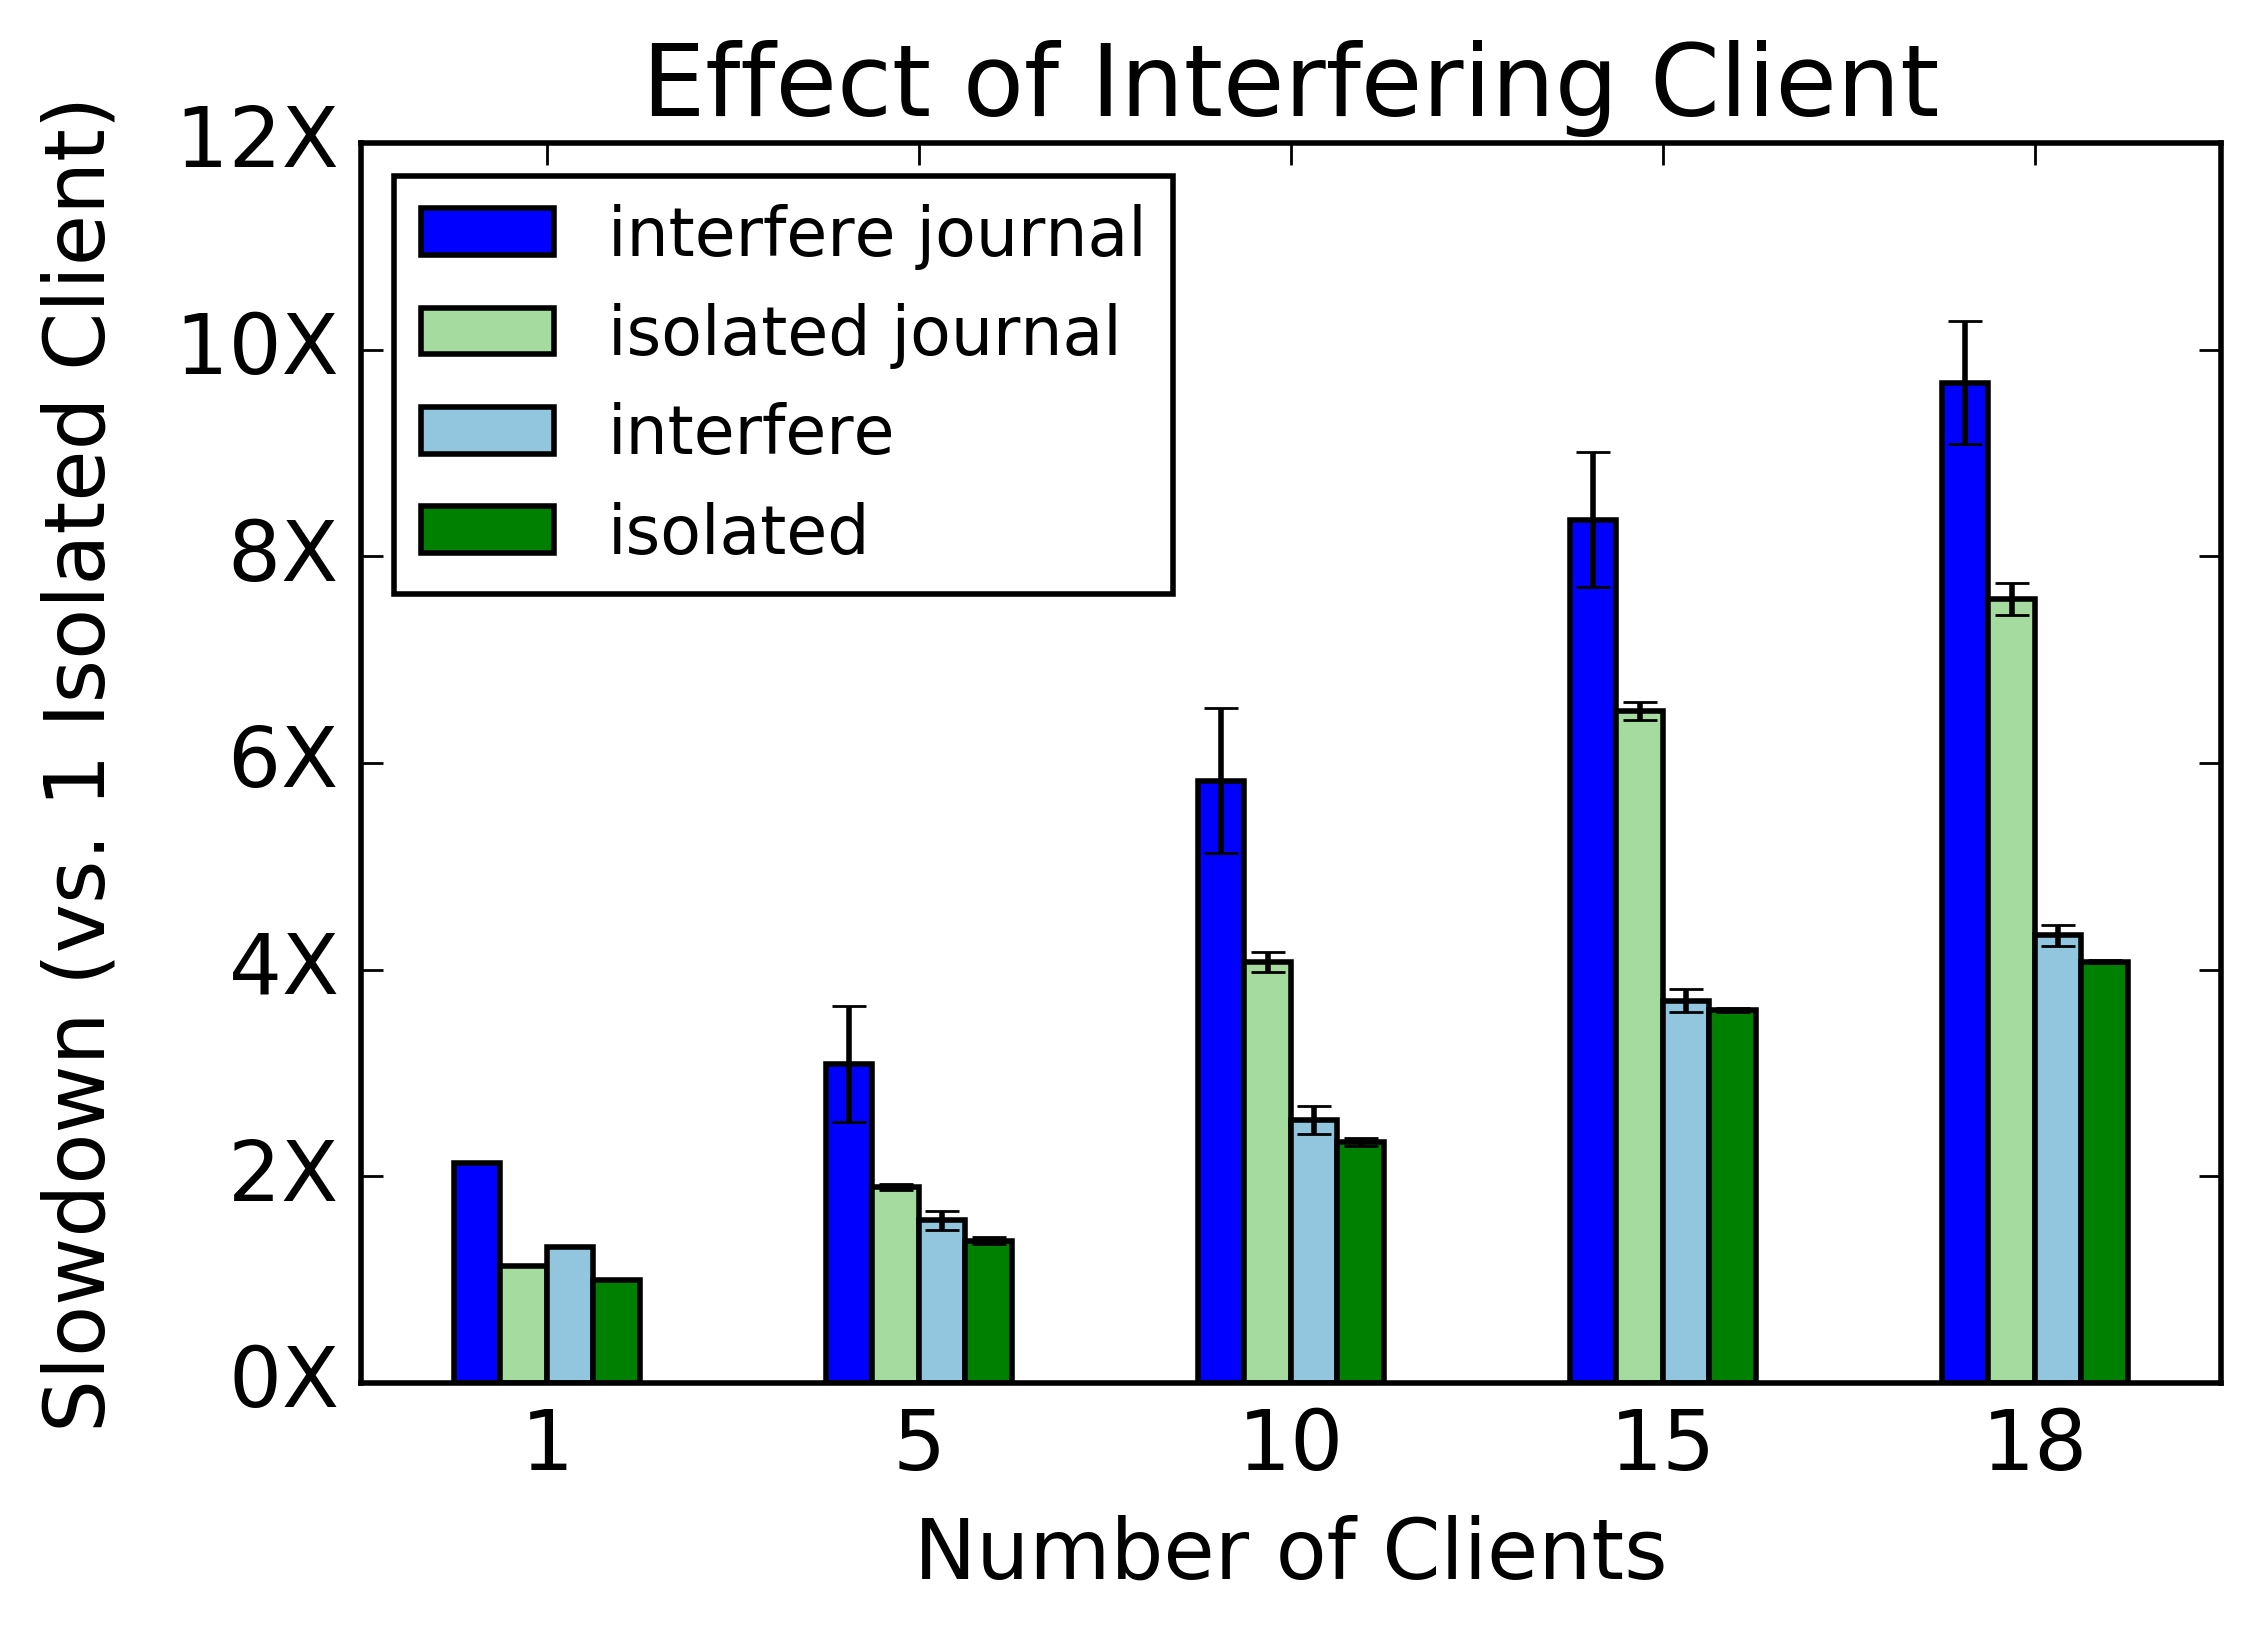
\includegraphics[width=0.98\linewidth]{graphs/slowdown-interfere-scale.png}
      \caption{[\href{https://github.com/michaelsevilla/cudele-popper/blob/master/experiments/baseline-creates/visualize/viz.ipynb}{source}]
      interference hurts variability}
      \label{fig:overhead-b}
  \end{subfigure}
  \begin{subfigure}[b]{.32\linewidth}
      \centering
      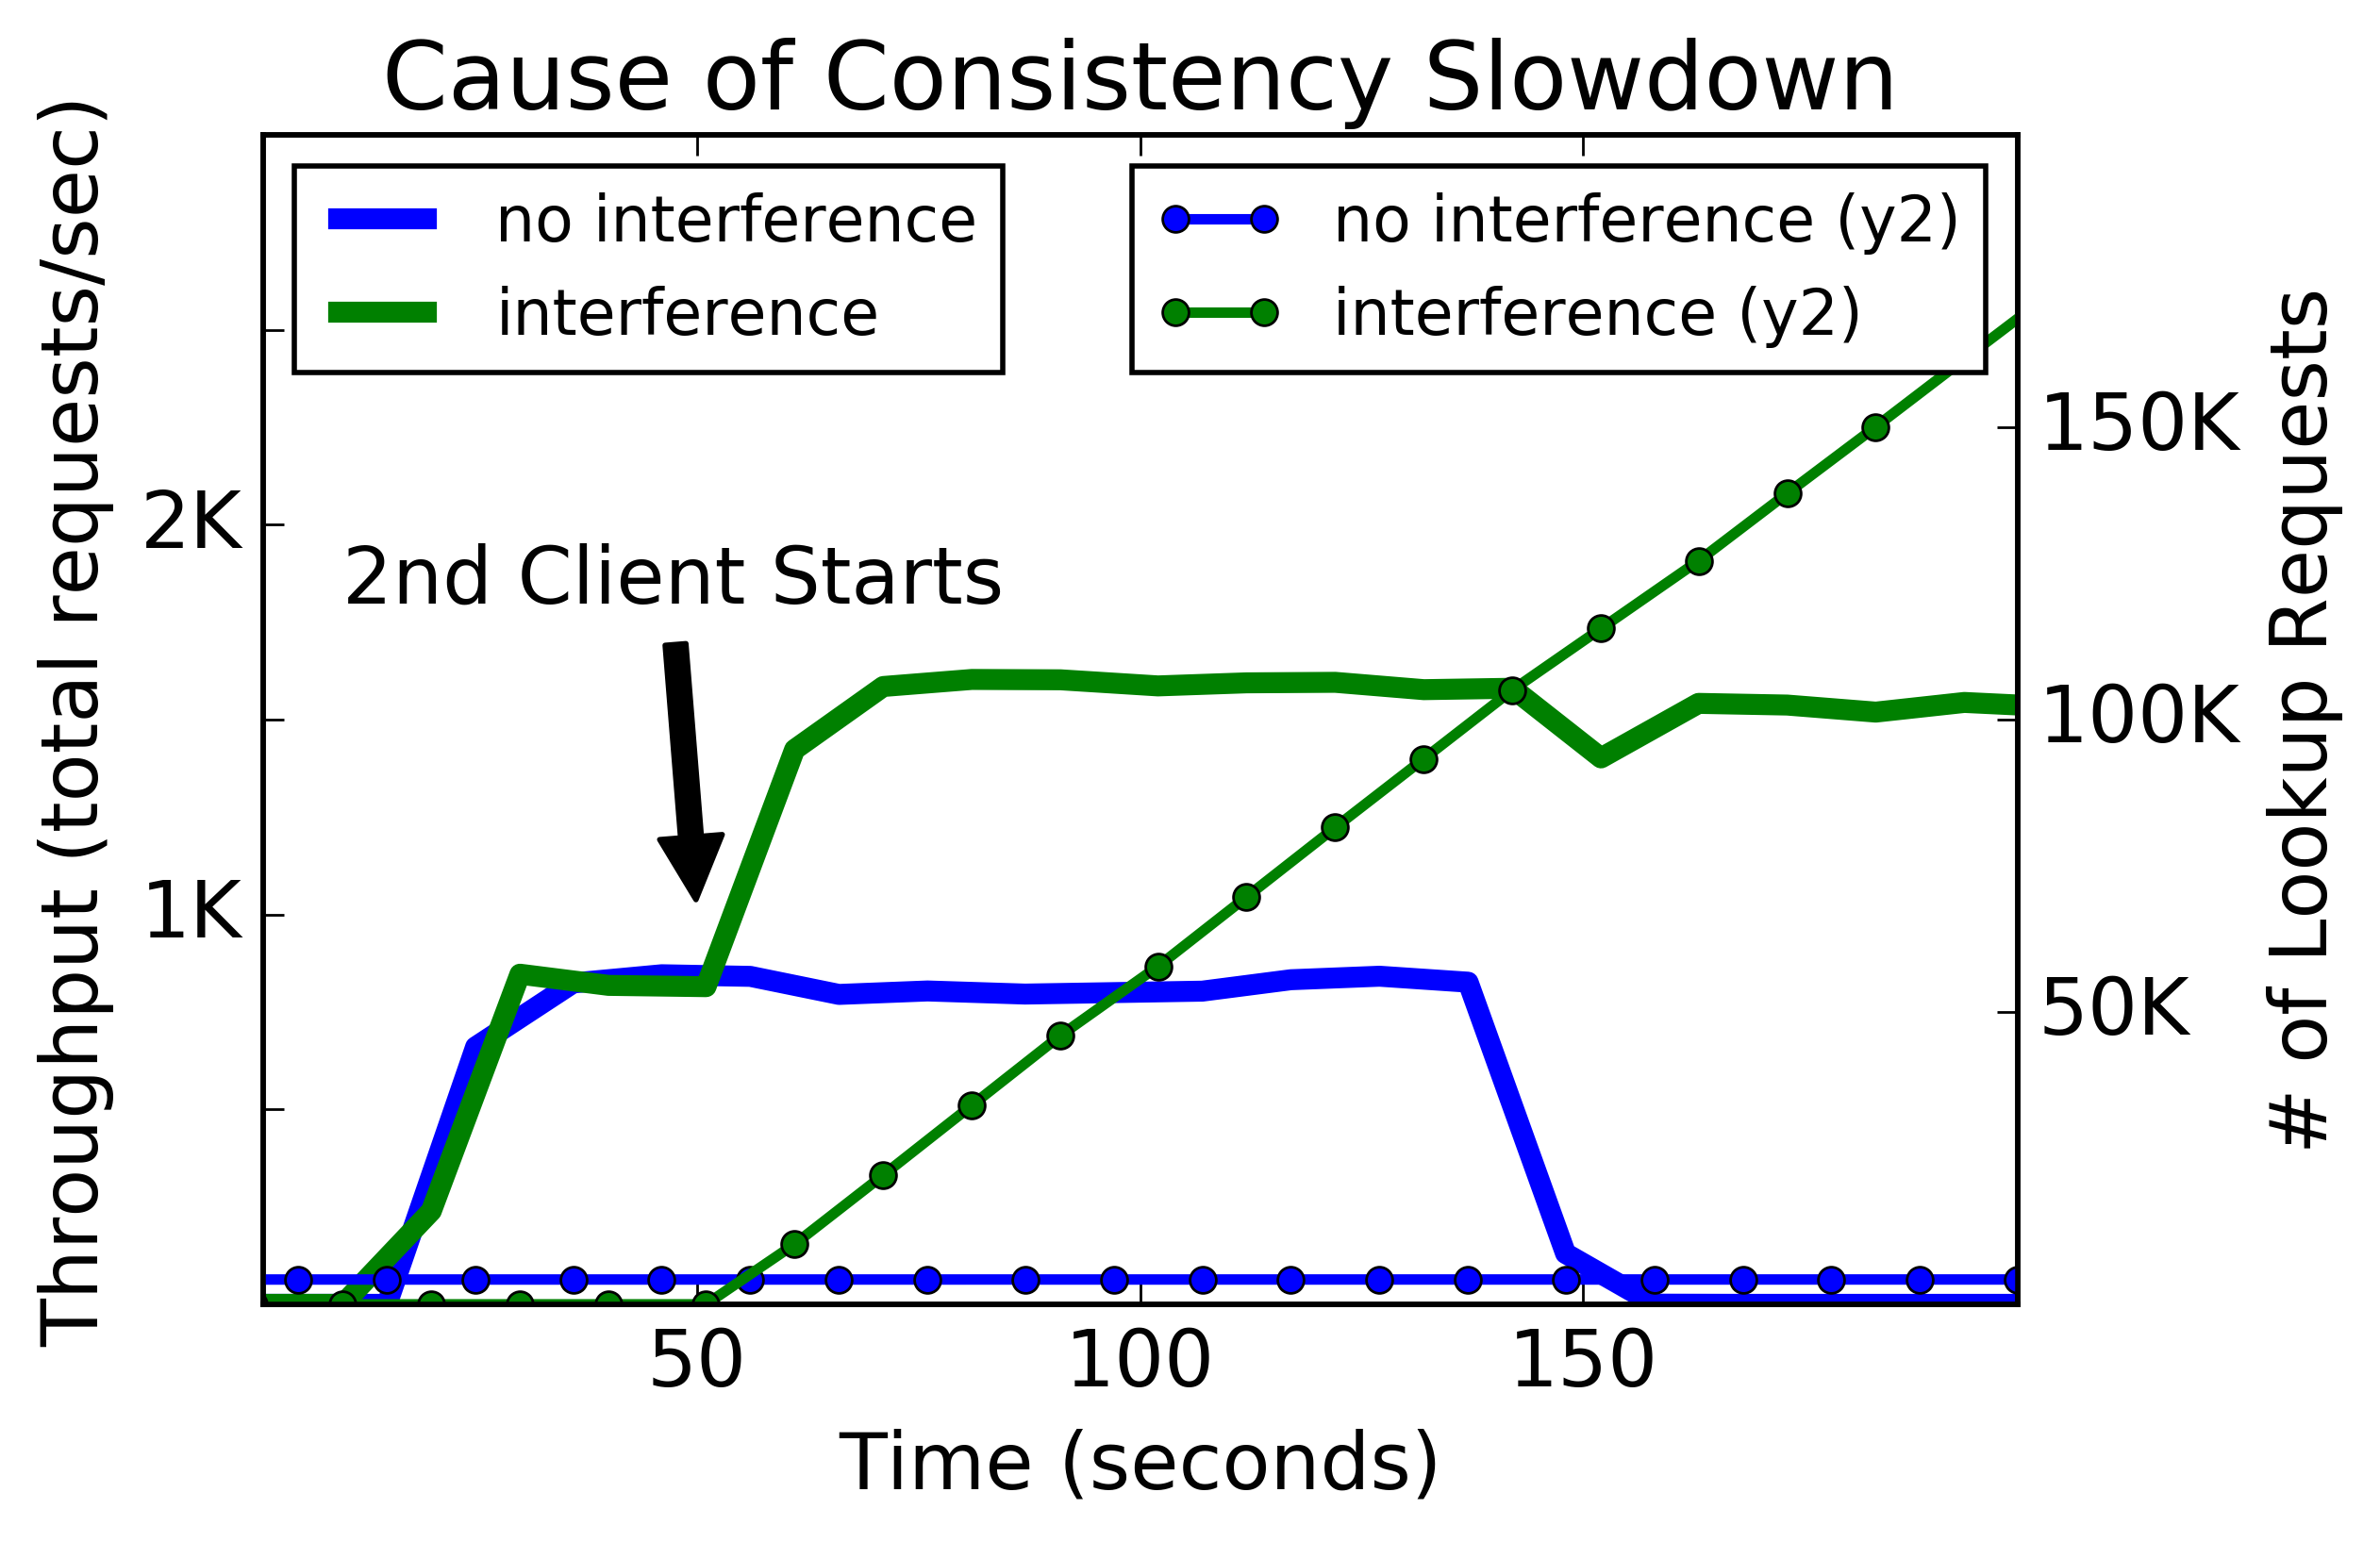
\includegraphics[width=1.15\linewidth]{graphs/behavior-interfere.png}
      \caption{[\href{https://github.com/michaelsevilla/cudele-popper/blob/master/experiments/baseline-interfere/visualize/viz.ipynb}{source}]
      interference increases RPCs}
      \label{fig:overhead-c}
  \end{subfigure}
  \caption{\newcomment{The durability and strong consistency slowdown of the
existing CephFS implementation increases as the number of clients scales.
Results in (a) and (b)  are normalized to 1 client that creates 100K files in
isolation.  (a) shows the effect of journaling metadata updates; ``segment(s)"
is the number of journal segments dispatched to disk at once. (b) shows the
slowdown when another client interferes by creating files in all directories
and (c) highlights the cause: }\oldcomment{The overhead of durability and
strong consistency in CephFS. (a) shows the effect of different journal segment
sizes, which are streamed into the object store for fault tolerance. (b) and
(c) show that} when another client interferes, capabilities are revoked and
metadata servers do more work.} \label{fig:overhead}
\end{figure*}

% what is durability
While durability is not specified by POSIX IO,
\oldcomment{users}\newcomment{administrators} expect that files they create or
modify survive failures.  We define three types of durability: global, local,
and none.  Global durability means that the client or server can fail at any
time and metadata will not be lost because it is ``safe" ({\it i.e.} striped or
replicated across a cluster). Local durability means that metadata can be lost
if the client or server stays down after a failure. None means that metadata is
volatile and that the system provides no guarantees when clients or servers
fail.  None is different than local durability because regardless of the type
of failure, metadata will be lost when components die in a None configuration.

% - sequential IO, trim redundant operations
\textbf{CephFS Design}: A journal of metadata updates that streams into the
resilient object store. Similar to LFS~\cite{rosenblum:acm1992-LFS} and
WAFL~\cite{hitz:wtec1994-WAFL} the metadata journal is designed to be large (on
the order of MBs) which ensures (1) sequential writes into the object store and
(2) the ability for daemons to trim redundant or irrelevant journal entries.
The journal is striped over objects where multiple journal updates can reside
on the same object. There are two tunables\newcomment{, related to groups of
journal events called segments,} for controlling the journal: the segment size
and the dispatch size ({\it i.e.} the number of segments that can be dispatched
at once).  Unless the journal saturates memory or CPU resources, larger values
for these tunables result in better performance.

% purpose of the journal
In addition to the metadata journal, CephFS also represents metadata in RADOS
as a metadata store, where directories and their file inodes are stored as
objects.  The metadata server applies the updates in the journal to the
metadata store when the journal reaches a certain size. The metadata store is
optimized for recovery ({\it i.e.} reading) while the metadata journal is
write-optimized.

%\begin{figure}[tb] \centering
%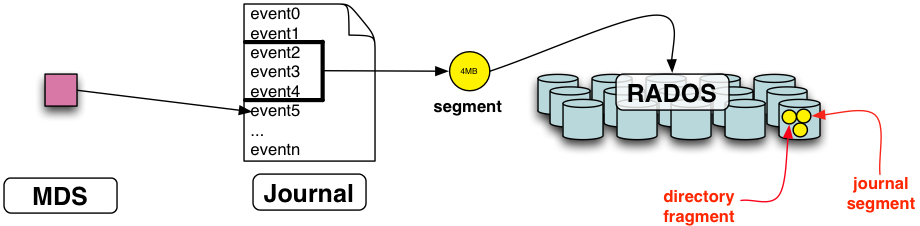
\includegraphics[width=1\linewidth]{./figures/journal.png} 
%\caption{CephFS has two views of the file system namespace: a journal of
%metadata updates and a metadata store. For fault tolerance, they are stored in
%the object store as segments and fragments, respectively.
%\label{fig:journal}}
%\end{figure}

% Effects on performance
Figure~\ref{fig:overhead-a} shows the effect of journaling with different
\oldcomment{segment sizes; the larger the segment size the bigger that the
writes into the object store are}\newcomment{dispatch sizes, normalized to 1
client that creates 100K files with journaling off (about 654 creates/sec). In
this case a dispatch size of 30 degrades performance the most because the
metadata server is overloaded with requests and cannot spare cycles to manage
concurrent segments.  Tuning and parameter sweeps show that a dispatch size of
10 is the worst and that larger sizes approach a dispatch size of 1; for all
future journal experiments we use a dispatch size of 40 which is a more
realistic configuration.  Although the ``no journal" curve appears flat, it is
actually a slowdown of about \(0.3\times\) per concurrent client; this slowdown
is a result of the peak throughput of a single metadata server, which we found
to be about 3000 operations per second}.  The trade-off for better performance
is memory consumption because a larger
\oldcomment{segment}\newcomment{dispatch} size uses more space for buffering.
\oldcomment{When journaling is on, the metadata server periodically stops serving requests
to flush ({\it i.e.} apply journal updates) to the metadata store.  The journal
overhead is sufficient enough to slow down metadata throughput but not so much
as to overwhelm the bandwidth of the object store.}

\textbf{Comparison to decoupled namespaces}: For BatchFS, if a client fails
when it is writing to the local log-structured merge tree (implemented as an
SSTable~\cite{ren:atc2013-tablefs}) then unwritten metadata operations are
lost. For DeltaFS, if the client fails then, on restart, the computation does
the work again -- since the snapshots of the namespace are never globally
consistent and there is no ground truth.  On the server side, BatchFS and
DeltaFS use IndexFS~\cite{ren:sc2014-indexfs}. IndexFS writes metadata to
SSTables, which initially reside in memory but are later flushed to the
underlying distributed file system.

\subsection{Strong Consistency}
\label{sec:strong-consistency}

Access to metadata in a POSIX IO-compliant file system is strongly consistent, so
reads and writes to the same inode or directory are globally ordered.  The
synchronization and serialization machinery needed to ensure that all clients
see the same state has high overhead.

% inode cache - reduces RPCs (lookups for create, readdirs for stats)

\textbf{CephFS Design}: Capabilities keep metadata strongly consistent. To
reduce the number of RPCs needed for consistency, clients can obtain
capabilities for reading and writing inodes, as well as caching reads,
buffering writes, changing the file size, and performing lazy IO.  To keep
track of the read caching and write buffering capabilities, the clients and
metadata servers agree on the state of each inode using an inode cache.  If a
client has the directory inode cached it can do metadata writes ({\it e.g.},
create) with a single RPC. If the client is not caching the directory inode
then it must do an extra RPC to determine if the file exists.  Unless the
client immediately reads all the inodes in the cache ({\it i.e.} \texttt{ls
-alR}), the inode cache is less useful for create-heavy workloads.

% benefits PROBLEM -- IS THIS THE METADATA PROTOCOL OR JUST THE OVERLOADEDNESS?
\oldcomment{This degradation is shown in Figure~\ref{fig:overhead-b}, where we
scale the number of clients and show the slowdown of the slowest client.  The
results are normalized to a single isolated client without a metadata server
journal and the error bars are the standard deviations of all client runtimes.}
\newcomment{Figure~\ref{fig:overhead-b} shows the slowdown of maintaining
strong consistency when scaling the number of clients.  We plot the slowdown of
the slowest client, normalized to 1 client that creates 100K files (about 513
creates/sec because the journal is turned back on).} For the ``interference"
curve, each client creates files in private directories and at 30 seconds we
launch another process that creates files in those directories. \oldcomment{18
is}\newcomment{20 clients has an asterisk\* because} the maximum number of
clients the metadata server can handle for this metadata-intensive workload
\newcomment{is actually 18}; at higher client load, the metadata server
complains about laggy and unresponsive requests.

\oldcomment{The benefits of caching the directory inode when creating
files}\newcomment{The cause for this slowdown} is shown in
Figure~\ref{fig:overhead-c}. The colors show the behavior of the client for two
different runs.  If only one client is creating files in a directory
(``no interference" curve on \(y1\) axis) then that client can lookup the existence of
new files locally before issuing a create request to the metadata server. If
another client starts creating files in the same directory then the directory
inode transitions out of read caching and the first client must send
\texttt{lookup()}s to the metadata server (``interference" curve on \(y2\) axis).
These extra requests increase the throughput of the ``interference" curve on the
\(y1\) axis because the metadata server can handle the extra load but
performance suffers.  



% TODO: what is the cost of trimming the cache?
% TODO: does CephFS still cache inodes when I turn off caching? Why is still keeping inodes in memory? Gah!

\textbf{Comparison to decoupled namespaces}: Decoupled namespaces
merge batches of metadata operations into the global namespaces when the job
completes.  In BatchFS, the merge is delayed by the application using an API to
switch between asynchronous and synchronous mode. The merge itself is explicitly
managed by the application but future work looks at more automated
methodologies. In DeltaFS, snapshots of the metadata subtrees stays on the client
machines; there is no ground truth and consistent namespaces are constructed
and resolved at application read time or when a 3rd party system ({\it e.g.},
middleware, scheduler, etc.) needs a view of the metadata. As a result, all the
overheads of maintaining consistency that we showed above are delayed until the
merge phase.
